\chapter{Introdução}
\label{chap:intro}

No Brasil, a eletricidade é gerada por hidrelétricas, termoelétricas, parques eólicos e usinas nucleares. Na maioria dos casos, devido a condições geográficas e de segurança, a energia gerada nem sempre é utilizada ou consumida no local de sua geração. Portanto, há a necessidade do uso de linhas de transmissão para transportar energia gerada na fonte geradora para a carga do consumidor \cite{rangel2009sistema}. O mercado consumidor brasileiro é composto de cerca de 47 milhões de unidades. Em termos de linhas de transmissão de energia, são cerca de 98.648,3 km, que devem estar operando 24 horas por dia, 7 dias por semana, 365 dias por ano e em perfeito estado de manutenção, para garantir eletricidade para os consumidores \cite{ons2013dados}

No Brasil, há uma quantidade considerável de linhas de transmissão de alta tensão que já ultrapassaram a vida útil as quais foram destinadas. Com o envelhecimento dos cabos, a inspeção para manutenção preventiva é um fator de extrema relevância para garantir o perfeito funcionamento dos sistemas elétricos. 
De um modo geral, as inspeções nas linhas de transmissão de alta tensão são realizadas regularmente de forma visual, a fim de identificar a necessidade da realização de manutenções preventivas. 
As inspeções buscam verificar a integridade física dos componentes das linhas, em termos de fissuras, corrosão e eventuais danos que venham a prejudicar o fornecimento de energia elétrica. Essas inspeções envolvem a análise da integridade estrutural das torres, da condição dos isoladores, das conexões das linhas de transmissão, dentre outros, a fim de se verificar a existência de eventuais pontos de ruptura. 

Um dos métodos empregados para detecção de pontos quentes nos cabos é o imageamento térmico, que é capaz de identificar uma elevação de temperatura nos cabos, o que é um indício de possíveis pontos de ruptura. A inspeção através de câmera térmica é uma importante ferramenta no campo das inspeções para manutenções preventivas. 
Outros pontos a serem inspecionados envolvem as condições do local onde as torres são instaladas, pois a vegetação e eventuais construções devem ser mantidas a uma distância mínima segura, tal que não ocorra nenhum contato entre quaisquer estruturas e as torres ou cabos de transmissão, evitando assim interferências no funcionamento da linha. 

Além disso, é essencial a garantia de dispor-se de um terreno em condições de trânsito de veículos para o transporte do pessoal de manutenção, transporte de ferramentas, dentre outros fatores. 
Durante vários anos, a inspeção de linhas de transmissão de alta tensão tem sido feita regularmente através de aeronaves tripuladas. As aeronaves executam vôos em baixa altitude e muito próximos das linhas de transmissão conforme mostrado nas  Figuras \ref{img:ihelic} e \ref{img:ihelichuma}.

%---------------picture------------------------------------
\begin{figure}[h!]												
	\centering												
	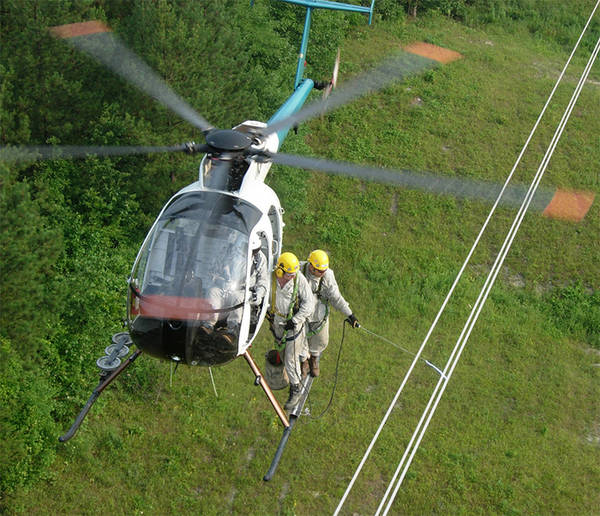
\includegraphics[width=0.6\textwidth]{./insphelic}				
	\caption{Inspeção de linhas de transmissão feita por aeronaves tripuladas.}	
	\label{img:ihelic}												
\end{figure}													
%----------------------------------------------------------
	
%---------------picture------------------------------------
\begin{figure} [h!]												 
	\centering													 
	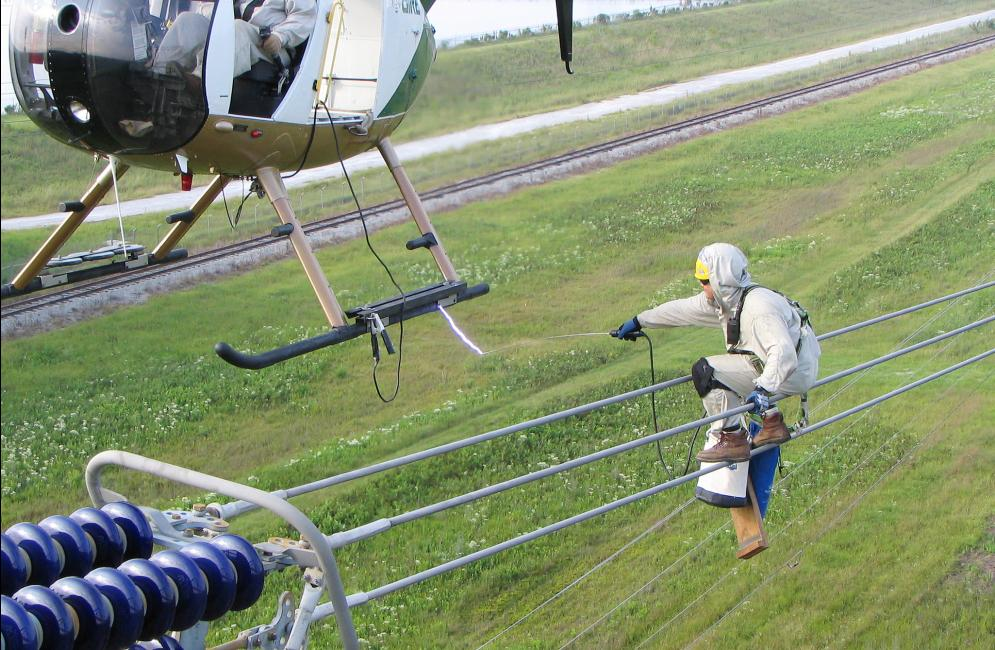
\includegraphics[width=0.6\textwidth]{./insphelichuma}				 
	\caption{Interação humana durante a inspeção de linhas de transmissão.}		
	\label{img:ihelichuma}												 
\end{figure}													 
%----------------------------------------------------------

Em alguns casos, devido às características geográficas da região, condições climáticas e outros fatores que venham a dificultar o sobrevôo, há uma grande exposição dos tripulantes a riscos associados à tarefa. Além dos perigos aos quais os tripulantes são expostos, a inspeção feita com aeronaves tem um custo bastante elevado. Outra forma alternativa de inspeção é o uso de veículos terrestres, porém essa forma é muito limitada, pois boa parte das linhas de transmissão está localizada em áreas de difícil acesso terrestre, muitas vezes restritas pelas características geográficas da região. Além disso, o ângulo de visão é, muitas vezes, desfavorável para a realização da inspeção.

%---------------picture------------------------------------
\begin{figure} [h!]												 
	\centering													 
	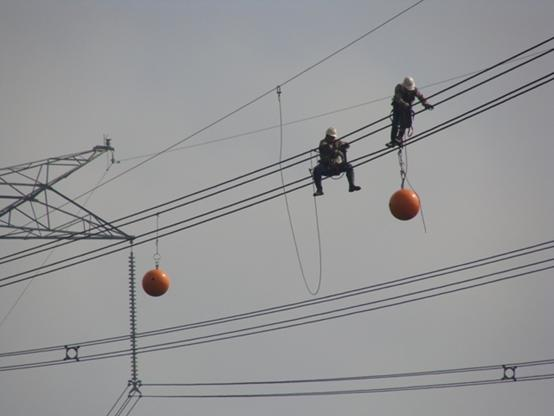
\includegraphics[width=0.6\textwidth]{./insphuma}				 
	\caption{Realização de inspeção em linhas de transmissão através da observação humana.}		
	\label{img:ihuma}												 
\end{figure}													 
%----------------------------------------------------------

Outra maneira de inspecionar as linhas de transmissão é através de eletricistas que literalmente caminham sobre os cabos de linhas de transmissão de alta tensão (Figura \ref{img:ihuma}), realizando inspeção visual e termográfica. Esse tipo de inspeção é lenta e não é viável, tendo em vista que o país possui milhares de quilômetros de linhas de transmissão.

Neste contexto vários robôs de inspeção de linhas de transmissão foram desenvolvidos, porém poucos deles consistiram em projetos de engenharia que sejam aplicáveis no mundo real, além disso a maioria eram robôs tele-operados, ou seja robôs controlados por seres humanos. Um dos pontos diferenciais deste projeto de tese é a proposição de um desenvolvimento de uma navegação autônoma utilizando técnicas de aprendizagem de máquinas até então não utilizadas em robôs de inspeção de linhas de transmissão de alta tensão.

%--------- NEW SECTION ----------------------
\section{Objetivos}
\label{sec:obj}

Desenvolver um protótipo de um robô de inspeção de linhas de transmissão

\subsection{Objetivos Específicos}
\label{ssec:objesp}

Desenvolver 4 funcionalidades para o robô, sendo elas:

\begin{itemize}
	\item Actuation: Funcionalidade responsável por atuar os motores que movimentam o robô.
	\item Motion Planning: Tem como objetivo planejar a movimentação das partes do robô
	\item Power Management: Responsável pelo gerenciamento e distribuição de energia para os componentes elétricos e eletrônicos do robô.
	\item System Integrity Check: Checagem da integridade do sistema antes do robô entrar em funcionamento.
\end{itemize}

%--------- NEW SECTION ----------------------
\section{Justificativa}
\label{sec:justi}
%O pesquisador/estudante deve apresentar os aspectos mais relevantes da pesquisa ressaltando os impactos (e.g. cient\'ifico, tecnol\'ogico, econ\^omico, social e ambiental) que a pesquisa causar\'a. Deve-se ter cuidado com a ingenuidade no momento em que os argumentos forem apresentados.

A inspeção de linhas de transmissão de alta tensão é uma tarefa difícil e altamente perigosa, atualmente esta inspeção é realizada através do auxílio de helicópteros os quais percorrem trajetórias próximas às linhas de transmissão e utilizam de câmeras termográficas as quais medem a temperatura nos cabos a partir da associação da quantidade de radiação emitida em determinada faixa de comprimento de onda com uma determinada temperatura. Porém os gastos com este tipo de inspeção são extremamente elevados, como consequência, as empresas responsáveis pela transmissão de energia não monitoram continuamente as condições dos cabos, e realizam inspeções nas linhas de transmissão em intervalos grandes. Outro modo de inspecionar as linhas de transmissão é através de eletricistas que literalmente andam sobre os cabos das linhas de transmissão de alta voltagem fazendo uma inspeção visual e podendo levar algum equipamento para medição de temperatura ao longo da linha, porém este tipo de inspeção é lenta e é inviável verificar milhares de quilômetros de linhas de transmissão utilizando este método.
Ambos os modos de inspeção de linhas de transmissão são arriscados, trazem perigos para as pessoas que estão a bordo do helicóptero; já que, este tem de voar próximo às linhas de transmissão e trazem perigos para o eletricista que irá andar sobre os cabos inspecionando-os visualmente ou com auxílio de algum equipamento, além de desconhecer-se completamente o efeito dos campos eletromagnéticos intensos desta região sobre a saúde destes eletricistas. Como consequência, realizar a inspeção de linhas de transmissão através da utilização de robôs móveis é algo que vem ganhando destaque no século XXI. Isto somente foi possível por causa dos avanços tecnológicos como sistema de localização global, os sistemas de transmissão de informação sem fio, a construção de micro-controladores mais baratos, rápidos e com maior capacidade de processamento, além dos grandes avanços que a computação e a microeletrônica têm obtido. Com isso as tarefas que seres humanos executam em ambientes insalubres, perigosos ou inóspitos poderão ser substituídas por uma mão-de-obra automatizada. Além disso, a aplicação da robótica móvel pode ser utilizada para a redução de custos.  No caso específico deste trabalho, a utilização de robôs de inspeção para linhas de transmissão atende a ambos os aspectos.
Um robô de inspeção de linhas de transmissão deve ser capaz de desviar de obstáculos como grampos de suspensão, grampos terminal passante, emendas a compreensão, emenda total pré-formada, tentos partidos, cabos amassados e dispositivos anti-vibração como amortecedores e festão. Estes obstáculos devem ser transpostos por sequências de movimentos executadas pelo robô. Além disso, idealmente o robô deve apresentar o menor peso, comprimento, altura, ter perfeita aerodinâmica, um formato desprovido de pontas, a maior autonomia possível, baixo custo, além de apresentar uma blindagem eletromagnética que deve impedir que os intensos campos magnéticos e elétricos, devido às elevadas correntes que passam nas linhas de transmissão, danifiquem os componentes eletrônicos, além disso, deve apresentar um sistema de comunicação wireless que não seja influenciado pelo elevado campo eletromagnético ao redor dos cabos, além de apresentar motores com elevado rendimento mecânico e elétrico, não apresentar derrapagem quando o mecanismo para movimentação das rodas for acionado, dentre outros.

Pagnano et. al \cite{pagnano2013roadmap} conclui que uma das principais buscas em futuros projetos devem estar centradas no desenvolvimento de detecção e transposição de obstáculos de forma autônoma, ou seja, não mais atribuir sequências de movimentos para os robôs mas desenvolver algoritmos de controle para que a detecção e ultrapassagem seja realizada de forma autônoma. Outro ponto a se observar é a completa abrangência de autonomia do robô durante sua navegação. 
  
Embora respondam por um número pequeno de ocorrências, se comparadas com as ocorrências em linhas de distribuição, um evento em uma linha de transmissão impacta de maneira desproporcionalmente mais severa, visto que a quantidade de clientes atendidos pelas linhas de transmissão é bem superior ao da linha de distribuição, afinal estas últimas são alimentadas pelas linhas de transmissão.

A manutenção preventiva é o procedimento mais adequado para aumentar a confiabilidade e evitar ocorrências indesejáveis em linhas de transmissão. No entanto, devido ao maior nível de tensão e conseqüentemente de maior escala das estruturas físicas da linha; efetuar a manutenção preventiva de maneira manual é uma tarefa muito difícil, custosa, por vezes requerendo o desligamento da linha. 

O uso de uma ferramenta automatizada para a inspeção destas linhas possibilitará uma redução no número e na freqüência de eventos em linhas de transmissão, aumentando a confiabilidade do sistema elétrico e reduzindo as perdas de energia; contribuindo para a melhoria do processo interno e a qualidade do serviço oferecido ao consumidor final, o que resulta em ganho financeiro para as concessionárias. Além deste benefício, é importante ressaltar que interrupções no fornecimento, mesmo que por curto espaço de tempo, têm como conseqüência impactos negativos sobre a sociedade e sobre a imagem da concessionária, sujeita à exposição na mídia.

Porém, a prática mostra que a idealização de soluções para os problemas levantados é algo distante da realidade, isto porque, além de ser fisicamente impossível de representar-se de forma exata situações ideais na prática; devido às perdas de energia e às inúmeras variáveis que teriam de ser abordadas para representar um problema de forma exata, mesmo que fosse possível construir um modelo muito próximo a realidade, o custo iria ser um dos fatores que iria inviabilizar a escolha dos melhores materiais e dos melhores dispositivos. Assim deve-se observar que, em geral, os robôs devem atender as características conforme certos requisitos de projeto, de modo que se aproxime ao máximo da condição ideal, desde que o custo permaneça abaixo de um valor aceitável. 


%--------- NEW SECTION ----------------------
\section{Requisitos do cliente}
\label{sec:reqc}
Foi especificado pelo cliente que o robô ELIR realize tais funções:

\begin{itemize}
	
	\item Transpor obstáculos e cadeia de isoladores;
	\item Deslocar-se através do consumo de baterias;
	\item Deslocamento/movimento realizada por servomotores;
	\item Realizar as funções de forma autônoma.
	
\end{itemize}




%--------- NEW SECTION ----------------------
\section{Organização do \thetypework}
\label{section:organizacao}

Este documento apresenta 5 capítulos e está estruturado da seguinte forma:

\begin{itemize}

  \item \textbf{Capítulo \ref{chap:intro} - Introdução}: Contextualiza o âmbito, no qual a pesquisa proposta está inserida. Apresenta, portanto, a definição do problema, objetivos e justificativas da pesquisa e como este \thetypeworkthree está estruturado;

  \item \textbf{Capítulo \ref{chap:concep} - Conceito do Sistema}: Conceitua o sistema por meio de diagramas que representam as arquiteturas do robô em diferentes níveis de abstração, abordando o estudo do estado da arte, desdobramento dos requisitos de qualidade e funcionamento do projeto.
  ;

  \item \textbf{Capítulo \ref{chap:mat} - Materiais e Métodos}: Mostra os materiais e métodos que foram utilizados durante o projeto, contendo a especificação de componentes, sendo eles softwares e dispositivos, assim como os esquemas elétricos e eletrônicos - e a descrição das funcionalidades;
  
  \item \textbf{Capítulo \ref{chap:result} - Resultados}: Exibe os resultados obtidos durante a confecção do projeto, apresentando os testes unitários e integrados, assim como as datas e quem o efetuou;
  

  \item \textbf{Capítulo \ref{chap:conc} - Conclusão}: Apresenta as conclusóes, contribuições
  e algumas sugestões de atividades de pesquisa a serem desenvolvidas no futuro.

\end{itemize}
